\documentclass[10pt,a4paper]{article}
\usepackage[margin=22mm]{geometry}
\usepackage{fontspec,amsmath,amssymb,amsthm,graphicx,xcolor,hyperref,fancyhdr}
\setmainfont{lmroman10-regular.otf}[BoldFont=lmroman10-bold.otf,ItalicFont=lmroman10-italic.otf,BoldItalicFont=lmroman10-bolditalic.otf]
\hypersetup{colorlinks=true,urlcolor=blue,linkcolor=blue}
\setlength{\parskip}{4pt}
\setlength{\parindent}{1.4em}
\newcommand{\norm}[1]{\left\lVert#1\right\rVert}
\newcommand{\sourcepagenumber}{editorial cover}
\newcommand{\SourcePage}[1]{\clearpage\gdef\sourcepagenumber{#1}}
\newenvironment{authorstatement}[1]{\par\medskip\noindent\textbf{#1}\ \itshape}{\par\medskip}
\newenvironment{authorremark}[1]{\par\medskip\noindent\textbf{#1}\ }{\par\medskip}
\pagestyle{fancy}\fancyhf{}\fancyhead[L]{\small Author text: original page \sourcepagenumber}\fancyhead[R]{\small Item 3005}\fancyfoot[C]{\thepage}\setlength{\headheight}{14pt}
\begin{document}\thispagestyle{plain}
\begin{center}
{\Large\bfseries 3005. Thompson's group $T$ has quadratic Dehn function}\par
\medskip
{\large Matteo Migliorini}
\end{center}
\noindent\textbf{Source and attribution.} Matteo Migliorini, ``Thompson's group $T$ has quadratic Dehn function,'' \emph{Forum of Mathematics, Sigma} \textbf{13} (2025), e109, pp.~1--13. DOI: \href{https://doi.org/10.1017/fms.2025.10075}{10.1017/fms.2025.10075}. Exact publisher version of record acquired 1 October 2026 at 14:57:48 UTC.\par
\noindent\textbf{Rights.} \copyright\ The Author(s), 2025. Published by Cambridge University Press. Original article licensed under \href{https://creativecommons.org/licenses/by/4.0/}{Creative Commons Attribution 4.0 International}. This editable TeX transcription reproduces author text and formulas from original pp.~1--8 through the complete Theorem A proof, and the original bibliography on p.~13. Figure~1 is an unchanged rendering crop of the author's diagram, with its caption transcribed below. Source running headers, acquisition footers, affiliation, abstract and publication administrative fields are excluded. Sections~5--6 and their separate generalized-group argument are outside this item's selected scope.\par
\noindent\textbf{Selected statement.} \emph{Theorem A. The Dehn function of Thompson's group $T$ is quadratic.} The precise group and coarse equivalence are the author's definitions in Section~2 below. Theorem~B appears only in the reproduced introduction as author context; this item counts the binary group $T$ alone.\par
\noindent\textbf{Difficulty.} H1. The author constructs finite-generator normal forms of linearly controlled length, then controls two- and three-rotation triangular loops by quadratic filling area. These dynamical normal-form and filling constructions exceed ordinary qualifying presentation manipulations; the established quadratic Dehn function of $F$ is a named prerequisite.\par
\noindent\textbf{Editorial transcription note.} All following mathematical statements, proofs and formulas are Matteo Migliorini's original English text in original order. This is assistant transcription, not native author TeX and not an assistant proof. Source wording and mathematical conventions are preserved, including the wording of Proposition~4.3; the original introduction supplies the nonhyperbolicity and lower-bound context for Theorem~A. Standard named external results are retained with the author's exact numbered references. No new mathematical explanation, formula repair or omitted proof is supplied.\par
\medskip
\noindent\textbf{Original source SHA-256}\par
\small\texttt{a675b6947f54e19f0b71ea2b413654f03919b8ae27e78af81104ee53c5e43af7}\normalsize
% Faithful transcription of author text; page provenance markers are editorial.
\SourcePage{1}
\section*{1. Introduction}
In 1965, Richard Thompson defined the three groups $F<T<V$ that are now known as Thompson's groups. They have been studied extensively in the last fifty years, as they arise naturally in many different areas of mathematics (geometric group theory and homotopy theory, to name a few). For a historical overview on Thompson's groups, we refer to the excellent survey by Cannon, Floyd and Parry [8].

Different points of view mean that Thompson's groups can be defined in many different ways. For example, one can define them combinatorially, as groups of certain partial automorphisms of a binary tree, or dynamically, as subgroups of homeomorphisms (with possibly some discontinuities, in the case of $V$) from the circle to itself.

Despite receiving a lot of attention, many questions about these groups are still open, the most famous arguably being whether $F$ is amenable.

Being finitely presented groups, an interesting problem is computing their Dehn functions. Indeed, the Dehn function is a natural quasi-isometric invariant associated to finitely presented groups; geometrically, it can be seen as the isoperimetric function associated to the presentation complex of the group.

Equivalently, one can also interpret the Dehn function combinatorially as the number of relations from the presentation that one needs to apply to reduce a word of length $n$ representing the identity to the empty word. In this sense, it is also related to the complexity of the word problem; for example, the latter is decidable if and only if the Dehn function is computable.

Note that the Dehn function of a finitely presented group is always either linear, in which case the group is hyperbolic [12], or it is at least quadratic [18].

The Dehn function of Thompson's group $F$ was proven by Guba [16] to be quadratic. While the lower bound follows easily from the fact that $F$ contains $\mathbb{Z}^2$ as a subgroup and is therefore not hyperbolic, the upper bound required a lot of work. Gersten first managed to prove an exponential upper bound [10] that was brought down to sub-exponential [15], then to $n^5$ [13], and finally to quadratic [16].

Thompson's groups $T$ and $V$ are also not hyperbolic, so their Dehn functions are at least quadratic. In fact, both are conjectured to have quadratic Dehn functions (see, for example, [21]). It was proven by Guba [14] that the Dehn functions of $T$ and $V$ have polynomial upper bounds of $n^7$ and $n^{11}$, respectively. The upper bound for $T$ was later improved to $n^5$ [20].

In this paper, we prove the conjecture for Thompson's group $T$.

\SourcePage{2}
\begin{authorstatement}{Theorem A.}
The Dehn function of Thompson's group $T$ is quadratic.
\end{authorstatement}
The proof relies on the fact that $F$ has quadratic Dehn function.

If in the combinatorial definition of Thompson's groups one replaces the binary tree with an $n$-ary tree, one gets three families of groups $F_n$, $T_n$, $V_n$. The family $V_n$ was introduced by Higman [17], while later, Brown [3] naturally extended the definition to $F_n$ and $T_n$; these groups are sometimes referred to as Higman--Thompson groups.

The same techniques used for proving Theorem A apply also for the family $T_n$.
\begin{authorstatement}{Theorem B.}
The Dehn function of the Higman--Thompson group $T_n$ is quadratic.
\end{authorstatement}
Here, we exploit the fact that by a result of Zhang [22], the groups $F_n$ have quadratic Dehn functions.

\subsection*{1.1. Strategy of the proof}
Thompson's groups $F$ and $T$ both have a finite and an infinite generating set that are well established in the literature; the advantage of the infinite one is that it admits a more symmetric (infinite) presentation.

Both groups admit normal forms, sometimes called $pq$ and $pcq$ factorization (see [8, Corollary 2.7, Theorem 5.7]), both of which use the infinite presentation; Guba used this normal form to prove that $F$ has quadratic Dehn function. For $T$, the situation is slightly more complicated: if we rewrite the normal form of an element of $T$ in terms of a finite generating set, the resulting word may be much longer than the actual norm of the element with respect to the word metric. Therefore, we introduce two different normal forms for $F$ and $T$ that use finite generating sets.

We look at Thompson's groups from the dynamical point of view, so $T$ is viewed as a certain subgroup of orientation-preserving self-homeomorphisms of the circle. If we parametrize the circle as the interval $[0,1]$ with the endpoints identified, then $F$ can be described as the subgroup of elements of $T$ that fix the point $0\equiv 1$. By considering the subgroup of elements that fix both $0$ and $\frac12$, we get a subgroup $H<F$ that is naturally isomorphic to $F\times F$.

We choose a finite generating set for $H$. From this, we construct a finite generating set for $F$ by adding an element $X_0\in F$ that does not fix $\frac12$. Similarly, from the generating set for $F$, we construct a generating set for $T$ by adding the rotation of the circle $C_0\in T$ of order two. By studying the dynamics of these groups $H<F<T$ on the circle, we can prove that every element of $F$ is represented by a word with at most one instance of $X_0$, and every element of $T$ is represented by a word with at most one instance of $C_0$. Such words are our chosen normal forms for $F$ and $T$; these are not unique, but this is not an issue for our purposes.

By a standard argument, it suffices to show that all triangular loops in the Cayley graph where the edges are normal forms have quadratic area. To perform this computation, we exploit the fact that in a triangular loop, almost all the letters are generators of $H$. Since $C_0$ stabilizes $\{0,\frac12\}$, it normalizes $H$; in fact, the generating set chosen for $H$ is invariant under conjugation by $C_0$. So we can commute the letter $C_0$ with every generator of $H$, by replacing the latter with its conjugate. This allows us to eliminate all instances of $C_0$ in the word, and then we conclude using that the Dehn function of $F$ is quadratic.

For Theorem B the strategy is similar, except now we consider the subgroup of $F_n$ that fixes all the points $\frac1n,\ldots,\frac{n-1}{n}$, and we work with the rotation of order $n$.

Note that one can prove Theorem B directly without proving the particular case for Thompson's group $T=T_2$. However, we choose to first give the proof for Theorem A, as the reader might be more familiar with Thompson's groups $F$ and $T$ than their generalizations, and the former have more established conventions for their generating sets. This makes the proof of Theorem A more explicit and hopefully easier to read, and in turn it helps to understand the proof of Theorem B.

\subsection*{1.2. Structure of the paper}
We start in Section 2 by recalling the definition of Dehn function, and we introduce Thompson's group $F$ and $T$, together with their generating sets, presentation, and some useful properties. In Section 3, we
\SourcePage{3}
\noindent show that $F$ admits a normal form with at most one instance of the generator $X_0$, and in Section 4, we introduce the normal form for $T$ that we use to prove Theorem A. In Section 5, we generalize all the arguments in the previous sections to prove Theorem B. We conclude with some remarks in Section 6.

\section*{2. Preliminaries}
We start by fixing some notation. Let $G$ be a finitely generated group, and $S=\{s_1,\ldots,s_k\}$ be a finite subset of $G$. If $w$ is a word in the alphabet $S\cup S^{-1}$, then we write $w(S)$ or $w(s_1,\ldots,s_k)$ to make the alphabet explicit. We denote the length of $w$ by $|w|$. If $g\in G$, and $S$ is a generating set, we denote by $\norm{g}_S$ the minimal length of a word representing $g$ (that is, the distance of $g$ from the identity with respect to the word metric). If the generating set is clear, we also write $\norm{g}_G$.

We say that a word $w(S)$ is null-homotopic if it represents the trivial element of $G$. If $G$ has a finite presentation $\langle S\mid\mathcal{R}\rangle$, and $w$ is a null-homotopic word, then $w$ can be written as a product of conjugates of $k$ relations, for some $k\in\mathbb{N}$; we call the minimum such $k$ the area of $w$, and denote it by $\operatorname{Area}(w)$.

The Dehn function of $G$ encodes the growth of the area in terms of the length of the word. More precisely, it is a function $\delta_G:\mathbb{N}\to\mathbb{N}$ defined by
\[
\delta_G(N)=\max\{\operatorname{Area}(w):w\text{ null-homotopic},\ |w|\le N\}.
\]
The Dehn function as defined above depends on the chosen presentation for $G$; to solve this problem, one introduces the following equivalence relation.

If $f,g:\mathbb{N}\to\mathbb{N}$, we say that $f\preccurlyeq g$ if there exists $C>0$ such that for all $N\in\mathbb{N}$, we have $f(N)\le Cg(CN+C)+CN+C$. If $f\preccurlyeq g\preccurlyeq f$, we write $f\asymp g$; different presentations of the same group (and more generally of quasi-isometric groups) have equivalent Dehn functions. A group $G$ has quadratic Dehn function if $\delta_G\asymp (N\mapsto N^2)$.

Throughout the paper, we identify the circle with the interval $[0,1]$ with the endpoints glued together. Thompson's group $T$ is the group of self-homeomorphisms of the circle that send dyadic rationals to dyadic rationals, are linear except on finitely many dyadic rationals, and the derivative is a power of $2$ (with integer exponent) wherever it is defined. The subgroup of $T$ consisting of the homeomorphisms that fix the point $0$ is Thompson's group $F$. We refer to [8] for an introduction on these groups.

Let $X_0,X_1,\ldots$ denote the standard generators of Thompson's group $F$. They are defined as follows:
\[
X_k(x)=\begin{cases}
x&\text{if }0\le x\le 1-\frac1{2^k},\\
\frac12\cdot x+\frac12-\frac1{2^{k+1}}&\text{if }1-\frac1{2^k}\le x\le 1-\frac1{2^{k+1}},\\
x-\frac1{2^{k+2}}&\text{if }1-\frac1{2^{k+1}}\le x\le 1-\frac1{2^{k+2}},\\
2x-1&\text{if }1-\frac1{2^{k+2}}\le x\le1.
\end{cases}
\]
Thompson's group $F$ admits both an infinite presentation
\[
\langle X_0,X_1,\ldots\mid X_jX_i=X_iX_{j+1}\text{ for all }i<j\rangle,
\]
involving all the $X_i$, with $i\in\mathbb{N}$, and a finite one with two generators $X_0,X_1$, given by
\[
\langle X_0,X_1\mid [X_0X_1^{-1},X_0^{-1}X_1X_0], [X_0X_1^{-1},X_0^{-2}X_1X_0^2]\rangle.
\]
In particular, all the other generators can be expressed in terms of the $X_i$ by the formula $X_{i+1}=X_0^{-i}X_1X_0^i$.

\SourcePage{4}
\begin{center}
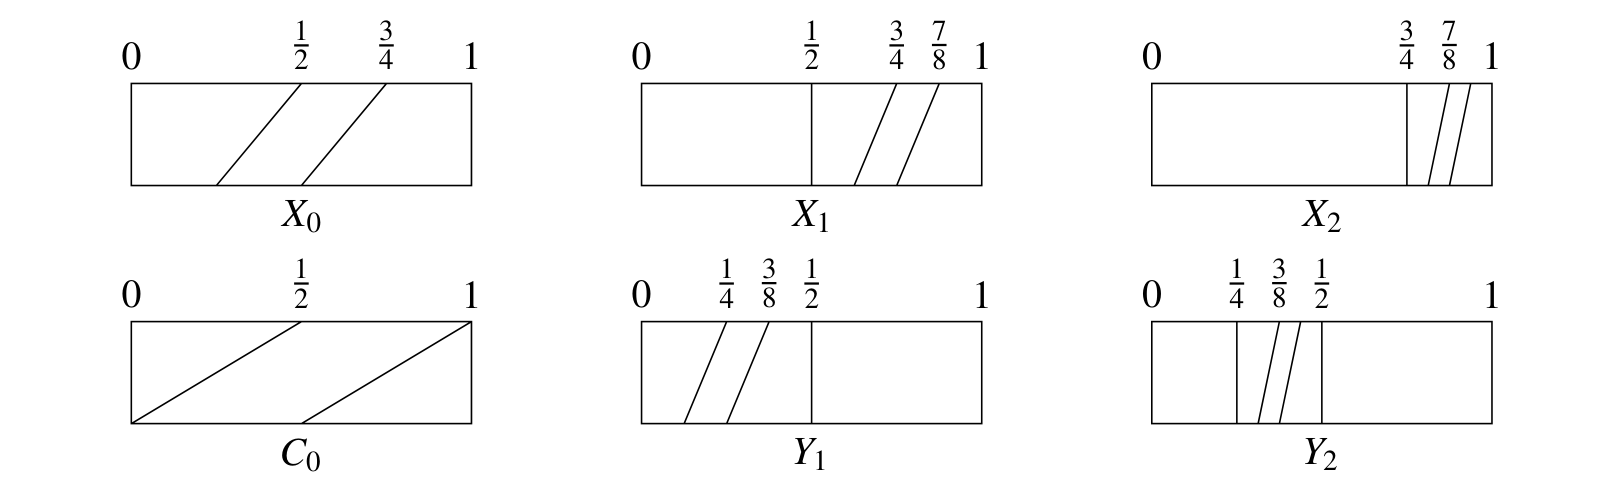
\includegraphics[width=.94\linewidth]{../assets/3005/figure1-original.png}\par
\smallskip
\textbf{Figure 1.} \emph{Rectangular diagrams for the generators $S_T$.}
\end{center}
To obtain a generating set for $T$, we need to add another homeomorphism that does not fix $0$. To this end, let $C_0$ be the homeomorphism defined by
\[
C_0(x)=\begin{cases}x+\frac12&\text{if }0\le x\le\frac12\\x-\frac12&\text{if }\frac12\le x\le1.\end{cases}
\]
In other words, $C_0$ is the rotation of the circle of order two.

\begin{authorremark}{Remark 2.1.}
One can also define elements $C_i$ of order $i+2$ for all $i\ge0$, as done in [8], and get an infinite presentation. To obtain a finite generating set, it suffices to add only one of the $C_i$ to the generators of $F$, and the usual choice is to use $C_1$ instead of $C_0$. To translate between the presentations found in the literature and the one we use here, it is helpful to keep in mind that $C_1=X_0^{-1}C_0$.
\end{authorremark}
We also define $Y_i:=C_0X_iC_0$ for $i\ge1$. Since $X_i$ has $\frac12$ as a fixed point for $i\ge1$, it follows that $Y_i\in F$. In this paper, we choose $S_F:=\{X_0^{\pm1},X_1^{\pm1},X_2^{\pm1},Y_1^{\pm1},Y_2^{\pm1}\}$ as a generating set for $F$, and $S_T:=S_F\cup\{C_0\}$ as a generating set for $T$. In Figure 1, we have drawn the rectangular diagrams for the generators: the top border represents the domain, while the bottom border represents the codomain (see [8] for more details).

\begin{authorstatement}{Lemma 2.2.}
Thompson's group $F$ admits the following presentation:
\[
\begin{gathered}
\langle S_F\mid [Y_1,X_1], [Y_1,X_2], X_0X_2=X_1X_0,\\
Y_1=X_0^2X_1^{-1}X_0^{-1},\ Y_2=X_0X_1^2X_2^{-1}X_1^{-1}X_0^{-1}\rangle.
\end{gathered}
\]
\end{authorstatement}
\begin{proof}
By using the rectangular diagrams, one can check that the relations hold in $F$. Moreover, one can use the last three relations to express $X_2,Y_1,Y_2$ in terms of $X_0,X_1$; after doing this, it turns out that the remaining two relations are conjugate to $[X_0X_1^{-1},X_0^{-1}X_1X_0]$, $[X_0X_1^{-1},X_0^{-2}X_1X_0^2]$, so the above presentation is equivalent to the standard presentation for $F$.
\end{proof}
The reason why we introduced these additional generators is that $\{X_1,X_2\}$ and $\{Y_1,Y_2\}$ generate two subgroups of $F$ that are both isomorphic to $F$ itself. More generally, given two dyadic numbers $0\le a<b\le1$ with $b-a=2^{-k}$ for some integer $k$, we may consider the subgroup of $F$ consisting of homeomorphisms that are the identity outside $(a,b)$; denote this group by $F[a,b]$.

\begin{authorstatement}{Theorem 2.3 [4, Theorem 3.1.3, 5.1.1].}
For all dyadic numbers $0\le a<b\le1$, the subgroup $F[a,b]$ is isomorphic to $F$ and undistorted.
\end{authorstatement}
In particular, $X_1,X_2$ generate $F[\frac12,1]$, while $Y_1,Y_2$ generate $F[0,\frac12]$; the element $C_0\in T$ conjugates $F[0,\frac12]$ to $F[\frac12,1]$ and vice versa, as we can see from the following.

\SourcePage{5}
\begin{authorstatement}{Lemma 2.4.}
Thompson's group $T$ is generated by the elements $S_T$ and satisfies the following relations:
\end{authorstatement}
\begin{enumerate}
\item $[Y_1,X_1]$,
\item $[Y_1,X_2]$,
\item $X_0X_2=X_1X_0$,
\item $Y_1=X_0^2X_1^{-1}X_0^{-1}$,
\item $X_0^{-1}Y_2X_0=X_1^2X_2^{-1}X_1^{-1}$,
\item $C_0^2=1$,
\item $(C_0X_0)^3=1$,
\item $C_0X_2=Y_2C_0$,
\item $C_0X_1=Y_1C_0$.
\end{enumerate}
\begin{proof}
The first five relations are the relations from $F$, while the last four can be checked directly by composing the homeomorphisms.
\end{proof}
\begin{authorremark}{Remark 2.5.}
It is possible to show that the above relations yield a presentation for $T$, as they can be obtained by manipulating the finite presentations for $T$ found in the literature [8, 7], but showing this equivalence by hand is a bit tedious. Luckily, we can avoid doing this computation: while proving that the Dehn function of $T$ is quadratic, we actually show that for some constant $C>0$, any null-homotopic word of length $n$ in the generating set $S_T$ can be reduced to the trivial word by applying at most $C\cdot n^2$ relations (1)-(9), which implies that the above is a presentation for $T$.
\end{authorremark}
\section*{3. A normal form for $F$}
Except for $X_0$, the generators for $F$ interact quite nicely with $C_0$, as $C_0X_i=Y_iC_0$ for $i\ge1$. The aim of this section is to show that every element of $F$ can be expressed as a word in the generators $S_F$ with at most one instance of $X_0$ (or its inverse). This defines a normal form for $F$, which will be very useful when computing the Dehn function of $T$.

Before doing so, we need some estimates on the word metric of $F$. An efficient way to estimate the word length is obtained by looking at the so-called reduced tree diagrams for elements in $F$ [5]. We translate this notion in terms of self-homeomorphisms of the interval.

Given $f\in F$, there exist subdivisions $0=x_0<\cdots<x_k=1$ and $0=y_0<\cdots<y_k=1$, with every interval $[x_i,x_{i+1}]$ and $[y_i,y_{i+1}]$ of the form $[\frac a{2^\ell},\frac{a+1}{2^\ell}]$, such that $f$ sends $x_i$ to $y_i$ and is affine on every $[x_i,x_{i+1}]$. If the subdivision is minimal, then the number of intervals $k$ is quasi-equivalent to the norm $\norm{f}_F$; that is, $\frac1Ck-C\le\norm{f}_F\le Ck+C$ for some constant $C>0$ independent of $f$.

From this, we get the following lemmas.
\begin{authorstatement}{Lemma 3.1.}
There exists a constant $C>0$ such that the following holds. Let $0<a=\frac d{2^k}<1$ be a dyadic number, with $d$ odd. There exists an element $f\in F$ such that $f(a)=\frac12$ and $\norm{f}_F\le C\cdot k+C$. Moreover, all $f\in F$ with $f(a)=\frac12$ satisfy $\norm{f}_F\ge\frac1Ck-C$.
\end{authorstatement}
\begin{proof}
There is a subdivision $x_0<\cdots<x_{k+1}$ where $x_j=a$ for some $j$; this can be constructed by iteratively bisecting the interval containing $a$. Then choose a subdivision $y_0<\cdots<y_{k+1}$ such that $y_j=\frac12$; the map associated to these subdivisions satisfies the requirements.

For the second statement, let $f\in F$ be any map with $f(a)=\frac12$, and choose subdivisions associated to $f$. Since $\frac12$ is a point of the second subdivision (unless $f$ is the identity), then $a$ must be a point of the first subdivision, and so the two subdivisions must have at least $k+1$ intervals; from this, we conclude.
\end{proof}
\begin{authorstatement}{Lemma 3.2.}
There exists $C>0$ such that the following holds. Let $0<a=\frac d{2^k}<1$ be a dyadic number, with $a\ne\frac12$ and $d$ odd. There exists an element $f\in F$ with $f(a)=\frac12$ that can be represented as a word of length at most $C\cdot k$ of the form
\end{authorstatement}
\SourcePage{6}
\[
\begin{array}{ll}
X_0\cdot w(X_1,X_2)&\text{if }a>\frac12\\
X_0^{-1}\cdot w(Y_1,Y_2)&\text{if }a<\frac12.
\end{array}
\]
\begin{proof}
If $a>\frac12$, by Lemma 3.1, we can obtain an element of $F$ that sends $2a-1$ to $\frac12$: by rescaling with $x\mapsto\frac12(x+1)$, we get $g\in F[\frac12,1]$ with $\norm{g}_{F[\frac12,1]}\le C(k-1)$ and $g(a)=\frac34$. If $w(X_1,X_2)$ is a shortest representative for $g$, then $X_0w(X_1,X_2)$ satisfies the hypotheses.

If $a<\frac12$, the construction is analogous by choosing $g\in F[0,\frac12]$ with $g(a)=\frac14$, and using $X_0^{-1}w(Y_1,Y_2)$.
\end{proof}
We are now able to show that elements of $F$ can be represented by words that have at most one instance of the letter $X_0$.

\begin{authorstatement}{Proposition 3.3.}
Let $f\in F$. Then $f$ is represented by a word $w(S)$ of the form
\[
\begin{array}{ll}
w=v(X_1,X_2)\cdot X_0^{-1}\cdot u(Y_1,Y_2)&\text{if }f^{-1}(\frac12)<\frac12\\
w=u(Y_1,Y_2)\cdot X_0\cdot v(X_1,X_2)&\text{if }f^{-1}(\frac12)>\frac12\\
w=v(X_1,X_2)\cdot u(Y_1,Y_2)&\text{if }f^{-1}(\frac12)=\frac12.
\end{array}
\]
Moreover, the word $w$ can be chosen of length bounded above by $C\cdot\norm{f}_F$, for some constant $C$ independent of $f$.
\end{authorstatement}
\begin{proof}
Let $a=\frac d{2^k}:=f^{-1}(\frac12)$; assume that $a>\frac12$. Let $f_1$ be the function with $f_1(a)=\frac12$ given by Lemma 3.2, represented by the word $X_0w_1(X_1,X_2)$ of length at most $C\cdot k$. By Lemma 3.1, this means that the length of $w_1$ is bounded linearly in terms of $\norm{f}_F$.

Since $f_1\circ f^{-1}$ fixes $\frac12$, then it belongs to the subgroup $F[0,\frac12]\times F[\frac12,1]$, which is undistorted by Theorem 2.3. There exists $f_2\in F[0,\frac12]$, $f_3\in F[\frac12,1]$, such that $f_1\circ f^{-1}=f_3\circ f_2$; let $w_2(Y_1,Y_2)$ and $w_3(X_1,X_2)$ be words representing $f_2$ and $f_3$, with
\[
|w_2|+|w_3|\le C'\cdot\norm{f_1\circ f^{-1}}_F\le C'\cdot(\norm{f}_F+\norm{f_1}_F),
\]
so the length of both $w_2$ and $w_3$ is bounded by a linear function of $\norm{f}_F$.

So $f=f_2^{-1}\circ f_3^{-1}\circ f_1$ is represented by
\[
w_2^{-1}(Y_1,Y_2)\cdot w_3^{-1}(X_1,X_2)\cdot X_0\cdot w_1(X_1,X_2).
\]
Finally, since for $\varepsilon\in\{\pm1\}$ we have
\[
X_1^\varepsilon X_0=X_0X_2^\varepsilon,\qquad X_2^\varepsilon X_0=X_0X_3^\varepsilon=X_0X_1^{-1}X_2^\varepsilon X_1,
\]
we obtain that $w_3^{-1}(X_1,X_2)X_0=X_0w_4(X_1,X_2)$ for some word $w_4$. Therefore, $f$ is represented by
\[
w_2^{-1}(Y_1,Y_2)\cdot X_0\cdot w_4(X_1,X_2),
\]
with $w_4$ bounded by a linear function of $\norm{f}_F$.

If $f^{-1}(\frac12)<\frac12$, then $f(\frac12)>\frac12$, so the result follows by applying the above on $f^{-1}$, and then taking the inverse at the end.

If $f(\frac12)=\frac12$, then we conclude by noting that $f\in F[0,\frac12]\times F[\frac12,1]$ and by using that the latter is an undistorted subgroup of $F$ by Theorem 2.3.
\end{proof}
\section*{4. The Dehn function of $T$}
The estimates for the word length based on tree diagrams hold for Thompson's group $T$ as well (see [7]). In particular, by the same arguments, we get the following.

\SourcePage{7}
\begin{authorstatement}{Lemma 4.1.}
There exists $C>0$ such that for every $f\in T$, if $f(0)=\frac d{2^k}$ with $d$ odd, then $\norm{f}_T\ge\frac1Ck-C$.
\end{authorstatement}
\begin{authorstatement}{Proposition 4.2.}
There exists $C>0$ such that every $f\in T\setminus F$ is represented by a word
\[
w=u(S_F)\cdot C_0\cdot v(S_F),
\]
such that $|w|\le C\cdot\norm{f}_T$.
\end{authorstatement}
\begin{proof}
Let $a=\frac d{2^k}:=f^{-1}(0)$. Let $f_1\in F$ be the element that sends $a$ to $\frac12$ given by Lemma 3.1. By Lemma 4.1, and since $F$ is undistorted in $T$ [7, Corollary 5.2], we have $\norm{f_1}_F\le C'\norm{f}_T+C'$ for some constant $C'$.

Now $f_2:=f\circ f_1^{-1}\circ C_0$ fixes the point $0$, so it belongs to $F$; moreover,
\[
\norm{f_2}_F\le C''\norm{f_2}_T\le C''(\norm{f}_T+\norm{f_1}_T+1).
\]
Since $f=f_2\circ C_0\circ f_1$, we may conclude by choosing short representatives $w_1(S_F),w_2(S_F)$ for $f_1,f_2$.
\end{proof}
We have shown that each element of $T$ is represented by a word containing at most one letter $C_0$, and whose length is bounded by a linear function of the norm of the element; we can employ these nice representatives to compute the Dehn function of $T$.

A standard argument, employed for example in [11, 9, 1], shows that it suffices to bound the area of triangular loops. This fact can be stated generally as follows:
\begin{authorstatement}{Proposition 4.3.}
Let $G=\langle S\mid\mathcal{R}\rangle$ be a finitely presented group, and for each $g\in G$, choose a subset $W_g$ of words in $S$ that represent the element $g$. Suppose that there exists $C>0$ such the following hold:
\begin{itemize}
\item[$\circ$] for every $g\in G$, there is $w\in W_g$ with $|w|\le C\cdot\norm{g}_G$;
\item[$\circ$] for every null-homotopic word $w=w_1w_2w_3$, with $w_i\in W_{g_i}$ for some elements $g_1,g_2,g_3$, we have that $\operatorname{Area}(w)\le C|w|^2$.
\end{itemize}
Then the Dehn function of $G$ is quadratic.
\end{authorstatement}
The set $W_g$ should be thought as some preferred word representatives for $g$. In our setting, the set $W_g$ consists of the word representatives for $g\in T$ that have at most one $C_0$; they exist by Proposition 4.2.

The proposition can be proven by subdividing a Van Kampen diagram for a generic loop into triangular cells, as explained in [9], or even directly by induction [1, Theorem 5.9]. Note that it is non-restrictive to prove the proposition for the case $|W_g|=1$ (that is, when using a unique normal form) as restricting every $W_g$ to a singleton can only weaken the hypotheses.

This simplifies our work considerably, as it suffices to compute the area of null-homotopic words containing up to three instances of $C_0$. Note that a word containing exactly one instance of $C_0$ cannot be null-homotopic, as it cannot send the point $0$ to itself. So there are just two cases to check.
\begin{authorstatement}{Proposition 4.4.}
There exists $C>0$ such that every null-homotopic word of the form
\[
w=C_0\cdot w_1(S_F)\cdot C_0\cdot w_2(S_F)
\]
has area at most $C\cdot|w|^2$.
\end{authorstatement}
\begin{proof}
Let $f_2\in F$ be the element represented by $w_2$ and $C_0w_1^{-1}C_0$. Since $C_0w_1C_0$ fixes the point $\frac12$, then $f_2$ can be represented by a word $u(X_1,X_2,Y_1,Y_2)$ of length bounded by $C|w_2|$, for some $C>0$. Therefore, using $\delta_F((C+1)\cdot|w_2|)$ many instances of relations (1)--(5), we can replace $w_2$ by $u$, obtaining the word
\[
C_0\cdot w_1(S_F)\cdot C_0\cdot u(X_1,X_2,Y_1,Y_2).
\]
\SourcePage{8}
\noindent Now using relations (8), (9), we can shift all letters in $u$ to the left of $C_0$, obtaining
\[
C_0\cdot w_1(S_F)\cdot u(Y_1,Y_2,X_1,X_2)\cdot C_0,
\]
where with $u(Y_1,Y_2,X_1,X_2)$, we denote the word obtained by $u(X_1,X_2,Y_1,Y_2)$ replacing $X_1\rightsquigarrow Y_1$, $X_2\rightsquigarrow Y_2$, $Y_1\rightsquigarrow X_1$ and $Y_2\rightsquigarrow X_2$ (note that $C_0X_1=Y_1C_0$ is conjugate to $C_0Y_1=X_1C_0$, since $C_0$ is an involution). After conjugating by $C_0$, we get a word in $S_F$. The result follows from the fact that $F$ has quadratic Dehn function [16].
\end{proof}
\begin{authorstatement}{Proposition 4.5.}
There exists $C>0$ such that every null-homotopic word of the form
\[
w=C_0\cdot w_1(S_F)\cdot C_0\cdot w_2(S_F)\cdot C_0\cdot w_3(S_F)
\]
has area at most $C\cdot|w|^2$.
\end{authorstatement}
\begin{proof}
Let $f_2\in F$ be the element represented by $w_2$. If $f_2(\frac12)=\frac12$, then it would follow that $w(0)=\frac12$, so $w$ did not represent the identity of $T$. Therefore, assume that $f_2^{-1}(\frac12)>\frac12$ (the other case is equivalent by taking the inverse of $w$), and let $u(Y_1,Y_2)\cdot X_0\cdot v(X_1,X_2)$ be the representative for $f_2$ given by Proposition 3.3.

We can replace $w_2$ by $u\cdot X_0\cdot v$ using a number of relations that is at most quadratic in $|w_2|$, since the Dehn function of $F$ is quadratic. We obtain
\[
C_0\cdot w_1(S_F)\cdot C_0\cdot u(Y_1,Y_2)\cdot X_0\cdot v(X_1,X_2)\cdot C_0\cdot w_3(S_F).
\]
Now use relations (8), (9) to shift $u$ to the left of $C_0$, and $v$ to the right of the other $C_0$. We get
\[
C_0\cdot w_1(S_F)\cdot u(X_1,X_2)\cdot C_0\cdot X_0\cdot C_0\cdot v(Y_1,Y_2)\cdot w_3(S_F).
\]
Using $(C_0X_0)^3=1$, we have that $C_0X_0C_0=X_0^{-1}C_0X_0^{-1}$. After this substitution, the word contains only two $C_0$ letters, so we conclude by the previous lemma.
\end{proof}
The proof of Theorem A is now complete.

\SourcePage{13 (bibliography)}
\section*{References}
\begin{enumerate}
\renewcommand{\labelenumi}{[\arabic{enumi}]}
\item D. Ascari, F. Bertolotti, G. Italiano, C. Llosa Isenrich and M. Migliorini, `Dehn functions of subgroups of products of free groups. Part II: Precise computations', Preprint, 2025, arXiv:2502.03180.
\item J.-C. Birget, `The groups of Richard Thompson and complexity', \emph{Internat. J. Algebra Comput.} \textbf{14}(05n06) (2004), 569--626.
\item K. S. Brown, `Finiteness properties of groups', \emph{J. Pure Appl. Algebra} \textbf{44}(1) (1987), 45--75.
\item J. Burillo, \emph{An Introduction to Thompson's Group $F$}, available at \url{https://web.mat.upc.edu/pep.burillo/F%20book.pdf}.
\item J. Burillo, `Quasi-isometrically embedded subgroups of Thompson's group F', \emph{J. Algebra} \textbf{212}(1) (1999), 65--78.
\item J. Burillo, S. Cleary and M. Stein, `Metrics and embeddings of generalizations of Thompson's group F', \emph{Trans. Amer. Math. Soc.} \textbf{353}(4) (2001), 1677--1689.
\item J. Burillo, S. Cleary, M. Stein and J. Taback, `Combinatorial and metric properties of Thompson's group $T$', \emph{Trans. Amer. Math. Soc.} \textbf{361}(2) (2009), 631--652.
\item J. W. Cannon, W. J. Floyd and W. R. Parry, `Introductory notes on Richard Thompson's groups', \emph{Enseign. Math.} \textbf{42}(3--4) (1996), 215--256.
\item W. Carter and M. Forester, `The Dehn functions of Stallings--Bieri groups', \emph{Math. Ann.} \textbf{368}(1) (2017), 671--683.
\item S. Gersten, `Thompson's group $F$ is not combable', Unpublished.
\item S. Gersten and H. Short, `Some isoperimetric inequalities for kernels of free extensions', \emph{Geom. Dedicata} \textbf{92}(1) (2002), 63--72, 2002.
\item M. Gromov, \emph{Hyperbolic Groups} (Math. Sci. Res. Inst. Publ.) vol. 8 (Springer, New York, 1987).
\item V. S. Guba, `Polynomial upper bounds for the Dehn function of R. Thompson's group $F$', \emph{J. Group Theory} \textbf{1}(2) (1998), 203--211.
\item V. S. Guba, `Polynomial isoperimetric inequalities for Richard Thompson's groups F, T, and V', In \emph{Algorithmic Problems in Groups and Semigroups} (Birkh\"auser, Boston, MA, 2000), 91--120.
\item V. S. Guba and M. V. Sapir, `The Dehn function and a regular set of normal forms for R. Thompson's group F', \emph{J. Aust. Math. Soc.} \textbf{62}(3) (1997), 315--328.
\item V. S. Guba, `The Dehn function of Richard Thompson's group F is quadratic', \emph{Invent. Math.} \textbf{163}(2) (2006), 313--342.
\item G. Higman, \emph{Finitely Presented Infinite Simple Groups} (Notes in Pure Math.) (Department of Pure Mathematics, Department of Mathematics, I.A.S., Australian National University, 1974).
\item A. Yu. Ol'shanskii, `Hyperbolicity of groups with subquadratic isoperimetric inequality', \emph{Int. J. Algebra Comput.} \textbf{1} (1991), 281--290.
\item X. Sheng, `Quasi-isometric embeddings from generalised Thompson's groups to Thompson's group T', \emph{Tokyo J. Math.} \textbf{45}(2) (2022), 451--465.
\item K. Wang, Z.-J. Zheng and J. Zhang, `The Dehn function of Richard Thompson's group $T$', Preprint, 2015, arXiv:1511.04148.
\item M. C. B. Zaremsky, `Open problems', available at\newline
\url{https://www.albany.edu/~mz498674/open_problems.pdf}.
\item J. Zhang, `The Dehn function of the generalized Thompson group is quadratic', \emph{J. Algebra} \textbf{428} (2015), 457--470.
\end{enumerate}

\end{document}
